\begin{document}    

\chapter{Related Works}
\label{related_works}

\section{Lexical Semantic Change}
Language is dynamic; it changes in the passage of time. Previous studies have shown that lexical semantic change is both linguistically and socially motivated \parencite{kutuzov2017tracing,kutuzov2018survey,hamilton2016cultural}.

Semantic change can be broadly understood as the ``reanalysis'' of a word \parencite[650]{fortson2017approach}, and recognizing different types of semantic change does not entail an absolute distinction of a certain type, but outlines the research foci of previous studies \parencites[650]{fortson2017approach}{traugott2017semantic}. \citeauthor{bloomfield1933language}'s (\citeyear{bloomfield1933language}) classification of semantic change highlights the denotative (broadening/narrowing), connotative (degeneration/elevation), intensity (hyperbole), figurative (metonymy/metaphor), and relational (synecdoche) aspects of a lexical item that undergoes semantic change. In \textcite[199-205]{semanticincrowley2010}, types of semantic change are distinguished from the driving forces behind semantic change. The former includes broadening, narrowing, bifurcation (split), and shift, while the latter includes hyperbole, metaphor, euphemism, interference, folk etymology, and hypercorrection. In terms of the co-existence of the old and new meanings, bifurcation or shift is determined by the absence of the original sense. Semantic shift is reflected in the cognate words from target languages, which do not come to have the new meaning. For instances of hyperbole, words in constant use become more and more neutral. Interference describes the semantic relations of synonyms or homonyms, other words are in place to avoid confusion in communication. \textcite[81]{traugott2001regularity} also points out that meaning change often occurs in the direction from concrete to abstract. Originally, a lexical item bears contentful meaning. During grammaticalization, grammatical or procedural meaning is enriched although the contentful one might persist.

The main types of semantic change — of which e.g. \textcite{traugott2017semantic} offers historical examples are as follows (quoted from \parencite[6]{giulianelli2019lexical}):

\begin{enumerate}[label={(\arabic*)},nolistsep]
\item broadening (or generalization): the extension of the range of concepts designated by a term, 
\item narrowing (or specialization): the contraction of the range of concepts designated by a term, 
\item metaphorization: the conceptualization of one referent in terms of another, guided by analogical reasoning and implying an unspoken simile, 
\item metonymization: a meaning transfer from one word to another, guided by spatial, temporal, or causal contiguity between the two referents, 
\item amelioration: the acquisition of or shift towards a positive connotation,
\item pejoration: the acquisition of or shift towards a negative connotation.
\end{enumerate}
\vspace*{\baselineskip}

Depending on the initial step of investigation, semantic change can be approached from a semasiological and onamasiological perspective \parencites[17]{geeraerts1997diachronic}[25]{traugott2001regularity}. A semasiological perspective highlights the direction from linguistic expression to concept, so meaning change is studied under the consideration of a lexeme in a fixed, predetermined form. Conversely, an onamasiological perspective starts from concept to linguistic expression, and thus meaning change is framed within a given concept expressed by a set of alternative words. Nonetheless, both of the two complementary paths lead to such important topics in lexicology as polysemy and sense relations.

Semasiologically, when a lexeme undergoes semantic change and additional meanings are gained, the different senses might gradually be perceived as unrelated to one another by the language users. That is, the lexeme first becomes polysemous, and then homonymous \parencite[25]{traugott2001regularity}. Onamasiologically, on the other hand, focuses on synonyms, near­synonyms, and name-­giving to connect lexical items with sense relations that exist and develop under a concept over time \parencite[17]{geeraerts1997diachronic}.

Polysemy, for instance, goes hand in hand with the semasiological view. It is described as ``families of related meanings'' in \textcite[11]{traugott2001regularity}, and serves as a foundation of generalizations of semantic change with recurring patterns. The co­-existence of older and newer meanings in a lexical item, along with the influence of multiple meanings on one another, brings about the dynamics of ``saliency'' \parencite[12]{traugott2001regularity}. Being polysemous with more than one single semantic reading is not only necessary but also omnipresent. In particular, synchronic polysemy is pointed out as an integral component among the driving forces of lexical semantic change, a phenomenon that is often explored in a diachronic vein \parencite{robertinvanhove2008}.

As a topic that has long interested scholars in semantics and historical linguistics, semantic change is a complicated phenomenon resulting from an interplay of polysemy, with subjectification \parencite{traugott2001regularity}, prototypicality \parencite{geeraerts1997diachronic}, and other contributing factors. Semantic change has been extensively studied because linguistic variations of language use are pervasive in the synchronic settings, and are amplified in a diachronic scope \parencite{semanticincrowley2010,bowern2019semantic}. The term ``brachychrony'' is even coined by \textcite{mair1998corpora} to refer to a time span of 10 to 30 years, indicating how the change of a linguistic feature can be delineated within a short time frame.

The Invited Inferencing Theory of Semantic Change (IITSC) is proposed by \textcite[34-40]{traugott2001regularity} to account for the actuation of meanings through recognition of different stages of a linguistic expression depending on whether intended meanings are coded or crystallized into commonly used implicatures. In other words, the degree of conventionality reflects the stages in which an expression is during a certain period of time. The more conventional or less context-specific an expression is, the more crystalized or coded the meaning is conveyed through this expression, which indicates that the expression has evolved in the later stages of the IITSC. Importantly, the meaning of an expression is not limited to only one, but a second reading often becomes more and more readily accessible as the coded meaning, and is then acceptable by the language community. For example, through expressions of temporal sequence, invited inferences of causality can arise.

Over time, semantic change follows a path from coded meanings to utterance­-token meanings to utterance-­type, pragmatically polysemous meanings (GIINs) to new semantically coded meanings. That is, a new meaning emerges as a creative, innovative instance of language use by an individual and does not yet spread to a wider language community, but remains more idiosyncratic. Slowly, it is likely that the new meaning is acquired socially with strengthened pragmatic impact, and the expression is then pragmatically polysemous. The final stage of the evolution cycle is for the expression to be semantically polysemous or coded, with the new meaning being the dominant or salient reading.

\textcite{geeraerts1997diachronic} puts forwards a conceptual framework that describes semasiological change motivated by the prototypicality theory. Extensionally, members of a semantic category do not have equal representativeness or typicality of the category, and their membership can even be uncertain if the member is highly peripheral. Intensionally, meanings of less typical members are received from the more salient meanings and can overlap, yet the salient meanings are not determined solely from one single cluster of attributes. Generally, the synchronic semantic structure of lexical categories echoes with the diachronic semasiological change. Diachronically, the more salient the meaning, the more stable it is. When semantic change takes place, the expansion of referential range denoted by a meaning is extended from the prototypical center to the peripheral area.

Consequently, the peripheral area will have less and less in common with the prototypical center. It is also possible that a meaning of a lexical item is a combination of features that do not belong to the same cluster at all. Meanwhile, considering the uncertain boundaries to be drawn for a lexical item, its semantic history might involve discontinuous appearance of an identical meaning that is temporally unrelated to each other rather than resulting from textual evidences that do not survive time.

Under this conceptual framework, the flexibility of meaning construction relies on the adaptability and dynamics of human cognition that groups and regroups meanings to meet the need of cognitive efficiency. Building upon the distinction between speaker-oriented and hearer-oriented process to avoid possible communicative misunderstanding in phonology, this framework adopts a similar notion that homonymic clashes are resolved with opportunities of semantic change, including a tendency toward prototypicality and morphological transparency while striking a balance for as many morphological uses as possible.

For language speakers, the construction of meanings is flexible and sensitive to the context of use, in which ambiguity is resolved or cancelled \parencite{miller1991contextual,harris1954distributional}. Additionally, the operation of metonymy is a mechanism that plays a practical role in meaning construction, for this mechanism allows a word to carry referential and conceptual meanings simultaneously \parencite{hilpert2019historical,nerlich2001serial}. From the perspective of semantic change, an understanding of metonymic change, specifically, builds upon the familiarity of the culture in which the language is spoken, and therefore the attested examples in literature exhibit a rich diversity \parencite[649]{fortson2017approach}.

Yet, the semantic history of a word might also unfold beyond the intuition of the language users.  It is recognized that synchronically distinct meanings, which speakers of the given time period find conceptually related, might suggest otherwise, as in \textit{bachelor}, for a relationship exists between ``experiencing'' and ``evoking'', and \textit{actually}, ``unexpectedness'' and ``elaboration'' \parencite[13]{traugott2001regularity}. On the other hand, synchronic convergence is also likely, as shown in instances of folk etymology, but not as common cross­-linguistically.

\section{The Concept of Home in Literature}
The concept of home has been extensively studied in (environmental) psychology, sociology, anthropology, architecture, and other fields of study \parencite{samanani2019house,mallett2004understanding,moore2000placing,sixsmith1986meaning}. Specialized topics on homelessness, journeying, migration, gender, and aging are also discussed. Previously, the meanings and concept of home are explored through questionnaires, interviews, and by examining quotes and literary works. When described using language, this concept becomes intertwined with such words as \textit{home}, \textit{house}, \textit{dwelling}, and \textit{family}, with these words used interchangeably \parencite{mallett2004understanding,sixsmith1986meaning}. Nonetheless, home is ``not only of belonging but also of potential alienation when attempts to make home fail or are subverted'' \parencite{samanani2019house}. The emphasized aspects of different word choices from literature can be summarized as follows: 

\begin{enumerate}
    \item \textit{House}: physical space, reification of material circumstances and home concept organization through its layout, furnishings, renovation, and decoration \parencite{samanani2019house}. For instance, Bourdieu compares how Kabyle people see the pair of light and dark to public and private, and asserts that a house ``reflect[s] structured worldview'' and ``reproduce[s] it'' \parencite{samanani2019house}. Furthermore, materiality facilitates the development of a sense of belonging \parencite{moore2000placing}.
    \item \textit{Family}: a structured social unit of living. A family is symbolic of marriage, kinship, togetherness, and homeliness \parencite{samanani2019house}. A household is established through the process of homemaking, and the feeling of rootedness, safety, and value is thus deepened \parencite{samanani2019house,moore2000placing}. On top of that, marriage consolidates the concept of home through physical renovation and expansion of the house. From generation to generation, reproduction of class and gender differences is also strengthened or challenged \parencite{samanani2019house,mallett2004understanding}.
\end{enumerate}

The most detailed analysis is provided by \textcite{sixsmith1986meaning}. The co-existing relationships of home are plotted as three regions of ``personal'', ``social'', and ``physical'', based on questionnaire responses, as shown in \fref{fig:home_regions}. The ``diversity'' of the meanings of home is the motivation behind the research by \textcite{sixsmith1986meaning}. Home exists as a physical entity. Through styling and living, the house is transformed into a home. Home can even be used to describe any level of existential space, including neighborhood, town, city, and country, as well as having cultural expression attached to the meanings of home. The phenomenologically-based research collects empirical evidence from questionnaires under the framework of the ``person-environment unity'' that incorporates referents of places and actual experiences lived by people \parencite{sixsmith1986meaning}.

\begin{figure}[H]
  \begin{minipage}{\textwidth}
    \centering
    \raisebox{-0.5\height}{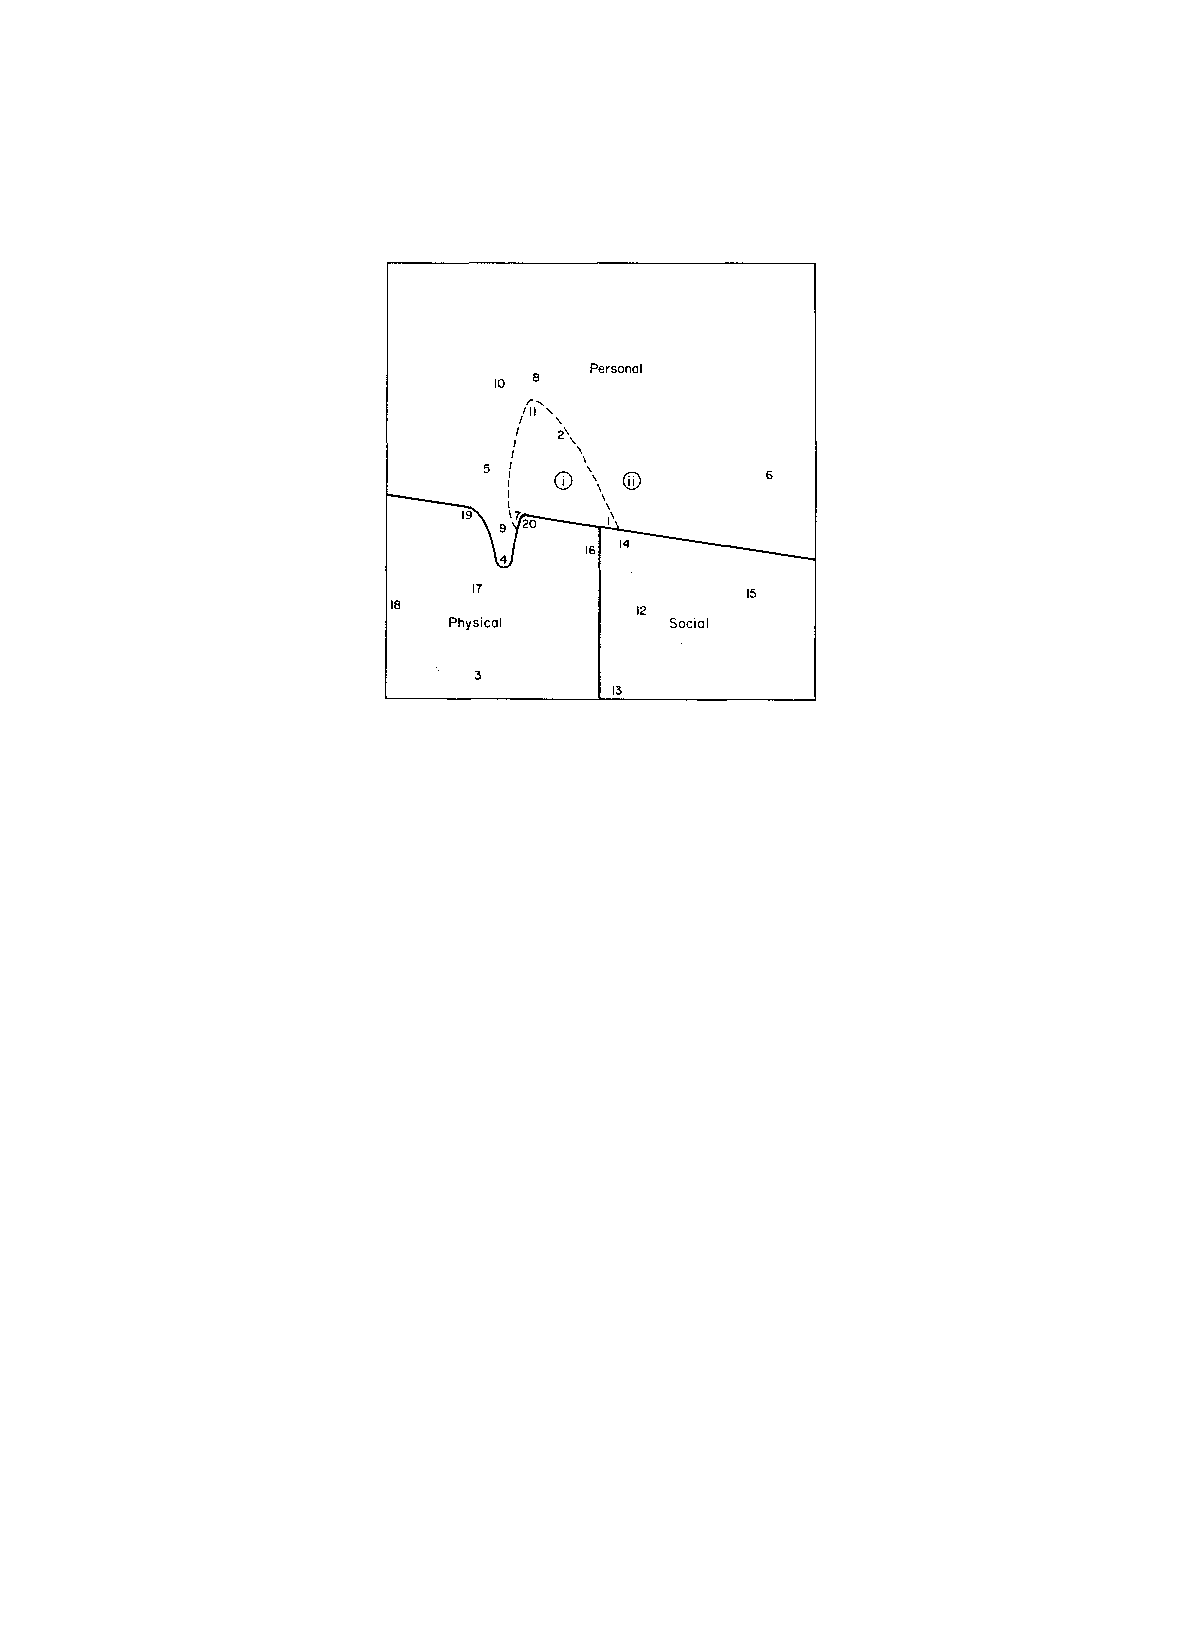
\includegraphics[width=0.45\textwidth]{figures_ref/Sixsmith_1986_regions_of_home.pdf}}
    \hspace*{.2in}
    \raisebox{-0.5\height}{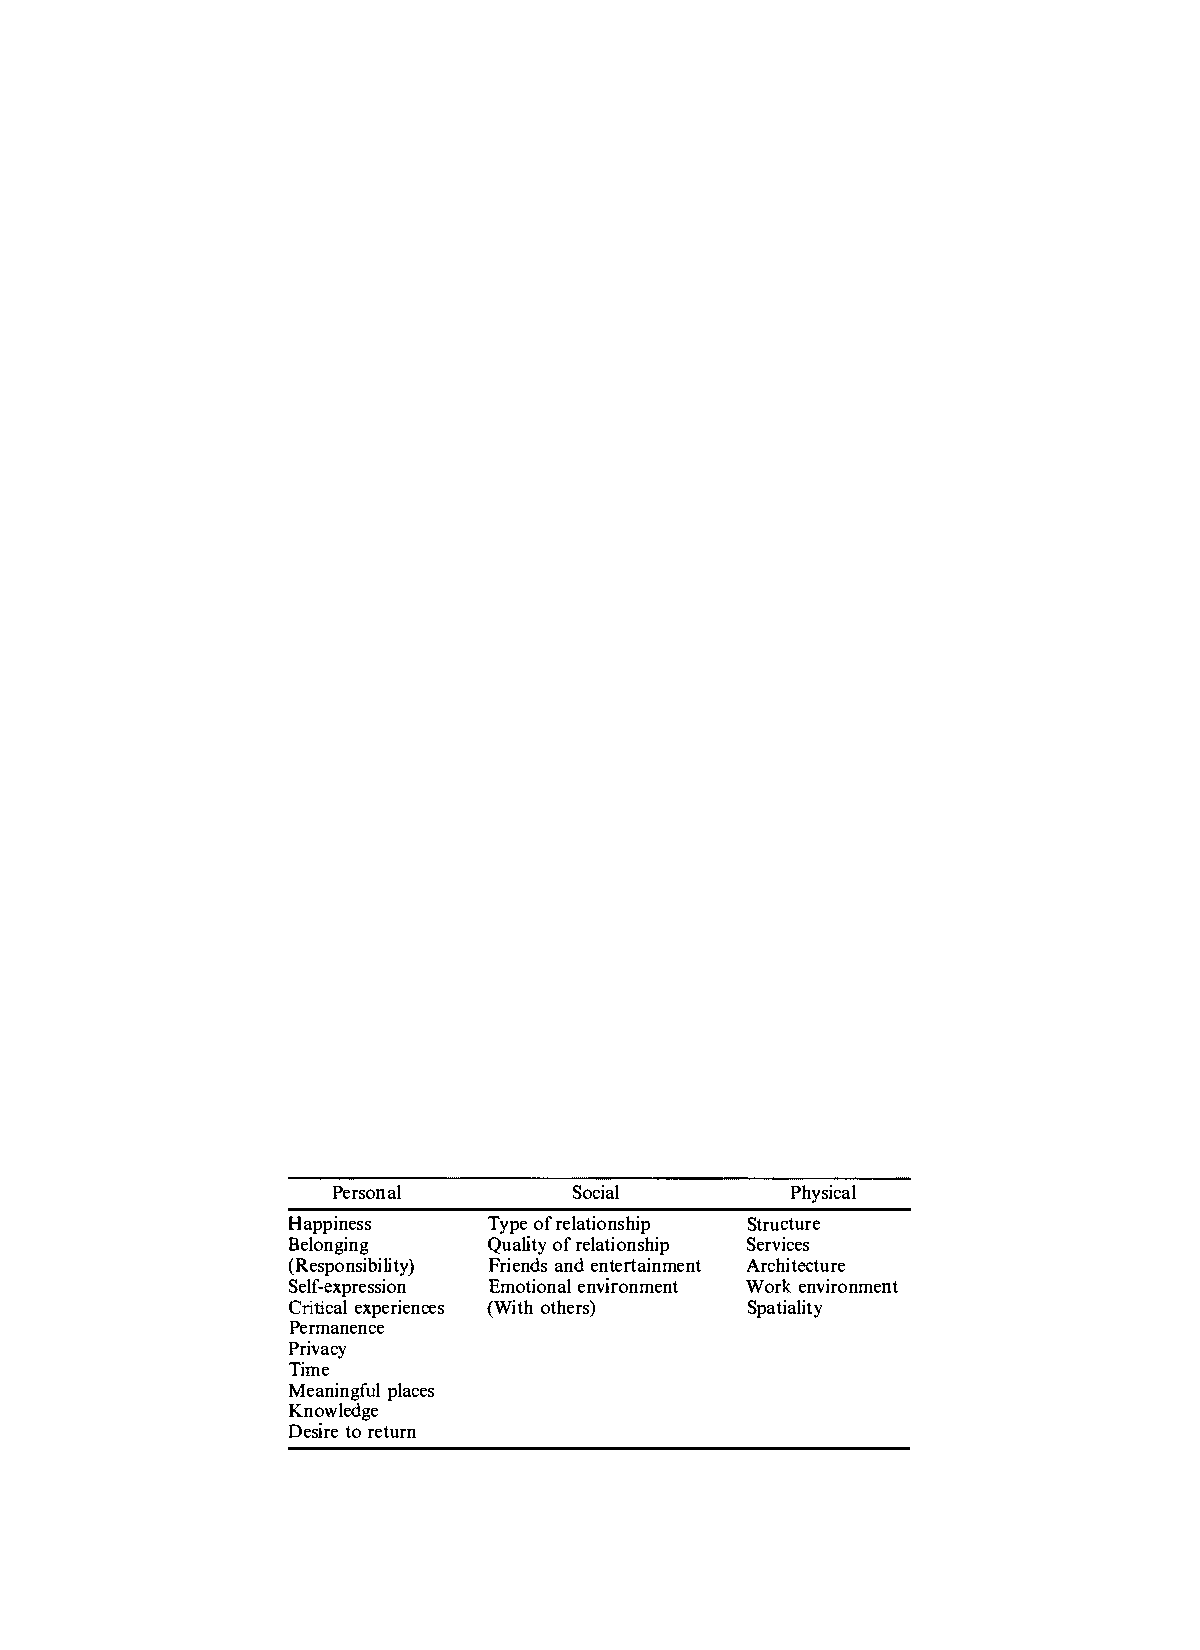
\includegraphics[width=0.45\textwidth]{figures_ref/Sixsmith_1986_categories_of_home.pdf}}
    \caption{The concept of home split into 3 regions (``Personal'', ``Physical'', and ``Social''). The spatial distribution of the 20 categories are derived from Kendall's Tau correlation between the meanings of home defined by participants  (Adopted from \textcite{sixsmith1986meaning}).}
    \label{fig:home_regions}
  \end{minipage}
\end{figure}

Through a method called ``multiple sorting task'', \textcite{sixsmith1986meaning} collects open-ended, participant-generated categories of home and sorting criteria. That is, the participants list categories of home and sort these categories according to a specific criterion they think of, and the procedure is repeated multiple times until all possible descriptions and orders have been attempted by the participants. This research is distinguished by the use of non-prescribed answers to depict the meanings of home from the perspective of the participants themselves. Through further transcription and categorization, the results have interwoven otherwise often disparate ideas of what home means statistically through multidimensional scaling technique.

Culturally, the concept of home in Taiwan as a physical space has undergone changes caused by the sway of the world order \parencite{沈孟穎2015台灣現代住宅設計之轉化}. Traditionally, \zh{合院}{héyuàn}{U-shaped courtyard homes} are common architectural forms reflecting Chinese analogy of an abode to an extension of the human figure and Chinese cultures of calligraphy and sculpture. Later, influenced by Japanese power, Japanese-Western Eclectic style was introduced to Taiwan, and \zh{街屋}{jiēwū}{town house;shop house} transforms the architectural landscape by incorporating the commercial use into the residential function. This hybridization is embodied and preserved in places like Dihua Street and Dadaocheng Area. Linguistically, \textcite{wang2005jia} have discussed the morphological development of \jia in pre-modern Chinese.

\section{Diachronic/historical Corpora}
The compilation of corpora to include historical texts and annotations enables more detailed linguistic analysis. Examples include
the Corpus of Historical American English (COHA, 1810-2010)\footnote{\url{https://www.english-corpora.org/coha/}},
A Representative Corpus of Historical English Registers (ARCHER, 1600-1999)\footnote{\url{https://www.projects.alc.manchester.ac.uk/archer/}},
Royal Society Corpus (RSC, 1665-1869)\footnote{\url{https://fedora.clarin-d.uni-saarland.de/rsc/}},
Corpus of Late Modern English Texts (CLMET, 1710-1920)\footnote{\url{https://perswww.kuleuven.be/~u0044428/}}, 
Hansard Corpus (1803-2005)\footnote{\url{https://www.english-corpora.org/hansard/}}, among many others.

In Chinese, the resources of diachronic corpora are relatively scarce, including Sheffield Corpus of Chinese\footnote{\url{https://www.dhi.ac.uk/scc/}} and 3 corpora compiled by Academia Sinica \parencite{wei1997corpus}--Academia Sinica Tagged Corpus of Old Chinese (中央研究院上古漢語語料庫, from pre-Qing to pre-Han)\footnote{\url{http://lingcorpus.iis.sinica.edu.tw/ancient/}}, Academia Sinica Tagged Corpus of Middle Chinese (中央研究院中古漢語語料庫, from late-Han to the Six Dynasties)\footnote{\url{http://lingcorpus.iis.sinica.edu.tw/middle/}}, and Academia Sinica Tagged Corpus of Early Mandarin Chinese (中央研究院近代漢語語料庫, from Tang to Qing)\footnote{\url{http://lingcorpus.iis.sinica.edu.tw/early/}}. The division into 3 corpora is based on the development of Chinese syntax to offer a synchronic sketch of Chinese and a basis for diachronic comparisons. In the 3 Academia Sinica tagged corpora, raw texts are available, with part of the texts imported from Scripta Sinica (漢籍全文資料庫計畫). It is also worth noting that the Google Books project for Chinese is not available until the year of 1950, and the latest date is 2008. It is believed that corpora creation is the foundation for a more thorough and accurate depiction for data collection during the establishment of lexical databases.

\section{Topics-Over-Time (TOT)}
Besides vector space models, topic models like Latent Dirichlet Allocation (LDA) are also widely applied to the study of semantic change, e.g., \textcite{wang2006topics}, \textcite{wijaya2011understanding}, and \textcite{hengchen2017phd}. As an extension to topic models, \acrlong{tot} (\acrshort{tot}) treats each year or each time slice as a document, and detects semantic change through top words used in documents and topics generated during the modeling. In practice, topic probability distribution is computed for each target word in the vocabulary of a specific time period, and word senses are derived from the topic distribution. Take the word \textit{gay} as an example. When the number of topics is set to 2, a trend of topic distribution change can be seen for the word, which echoes with the meaning change of the word from happiness or cheerfulness as an adjective, to homosexuality.

In companion with topic models, clustering methods like $k$-means clustering are insightful when the topic density of each cluster of a given time period is examined \parencite{wijaya2011understanding}. The results of $k$-means clustering show that top words with the highest tf-idf scores do not belong to the same clusters, indicating that these words are diverse in meaning contribution. Specifically, the clusters for the word \textit{awful} do not represent meaningful topics, which might be attributable to the fact that the word is used as an adverbial intensifier with general meaning. Over time, the word comes to be associated with negativity in meaning, and then less intensity is expressed through the use of the word. Another example is the word \textit{mouse}. By decreasing the $k$ in $k$-means, two clusters can be merged, and the last cluster represents the additional meaning acquired with the word.

Ultimately, the evolution of dynamic networks, specifically temporal exponential random graph model (ERGM) \parencite{robins2007introduction,wijaya2011understanding} is proposed to model the network of word co-occurrence in a diachronic vein. The word co-occurrence network illustrates the connections of words as nodes in the graph. A use case is to identify change of connotation in meaning for words such as \textit{awful}, for the co-occurrence network would justify that no connections exist among the nodes and thus these words do not belong to the same topic. On top of that, the emergence or disappearance of sub-graphs is indicative of newly-acquired or lost meanings of a word. The setting of lower weighting for sub-graphs also conforms with the possibility that the original meanings still prevail with the passage of time. In summary, the sketching of word profiles by selecting relevant metrics (i.e., tf-idf scores), the merging of clusters by adjusting the number of clusters, as well as the formation of the word co-occurrence network by building links and sub-graphs, have paved the way for early studies of semantic change modeling.

Recently, topic models continue to be used to explore the phenomenon of semantic change, yet with a different aim and approach. Topic models are used to yield topics that are most common in a given time period in order to anchor words that should be evaluated for the results \parencite{antoniak2018evaluating}. By so doing, the number of topics set for the identification of anchoring words are much larger than that for the \gls{tot} so that the computed mean probability is based on as diverse topics as possible.

\section{Diachronic Word Embeddings}
Recently, the application of computation to larger sets of words across longer periods of time enables the generalization of regularities on semantic change \parencite{hamilton2016law}. Diachronic word embeddings can be used to discover more possibilities of unknown change cases and underlying causes of general semantic change \parencite{hamilton2016cultural,kutuzov2017tracing,heuser2017word}. Semantic change driven by technological innovations are prominent examples, while shifts of meanings with linguistic cause tend to occur relatively more slowly \parencite{hamilton2016law}. The changes encompass changes to ``core meanings of words'' or ``subtle shifts of cultural associations'' \parencite{hamilton2016cultural}. The term ``brachychrony'' is even coined by \textcite{mair1998corpora} to refer to a time span of 10 to 30 years, indicating how the change of a linguistic feature can be delineated within a short time frame. A list of example use cases of semantic change modeling is provided in \tref{tab:use_case}.

\begingroup
\renewcommand{\arraystretch}{0.8}
\begin{threeparttable}[H]
  \centering
  % \captionsetup{justification=centering,margin=2cm}
  \caption{Example case studies of semantic change through computational analysis from literature}
  \label{tab:use_case}
  \begin{tabularx}{\textwidth}{lp{7.5cm}}
    \toprule
      \multicolumn{1}{c}{Literature} &
      \multicolumn{1}{c}{Use cases} \\ %& focus \\
    \midrule
      \textcite{kulkarni2015statistically} & apple, tape \\ %
      % & time point detection and cross-domain analysis \\
      \textcite{hamilton2016cultural} & actually, must, promise, gay, virus, cell \\ %
      % & cultural and linguistic shift \\
      \textcite{hamilton2016law} & gay, broadcast, awful, 病毒`virus' \footnotesymbol \\ %
      % & correlation with observed frequencies and polysemies\\
      \textcite{kutuzov2017tracing} & war, peace, stable \\ %
      % & monitoring world events\\
      \textcite{rodda2017panta} & πνεῦμα `breath' \textrightarrow\space `spirit' (Ancient Greek) \\ %
      % & exploration in Ancient Greek \\
      \textcite{antoniak2018evaluating} & marijuana \\ %
      % & word associations in different corpora \\
      \textcite{rudolph2018dynamic} & intelligence, iraq, jobs, prostitution \\
      \textcite{yao2018dynamic} & apple, amazon, obama, and trump \\
      \textcite{hu2019diachronic} & please, alien \\ %
      % & contextualized embeddings with sense inventories \\
      \textcite{rodina2020elmo} & провальный `a place where the surface collapsed inward' or `loss of consciousness' \textrightarrow\space `failed' (Russian) \\
    \bottomrule
  \end{tabularx}
  \begin{tablenotes}
    \linespread{1}\footnotesize
    \item[*]\hspace*{-\fontdimen2\font}A list of attested historical shifts is provided in \textcite{hamilton2016law}, and entries with the `obsolete' tag in the Oxford English Dictionary (OED) are also considered informative of records of meaning shifts.
  \end{tablenotes}
\end{threeparttable}
\endgroup
% source: https://tex.stackexchange.com/questions/229289/arrow-in-text-mode
% провальный

\vspace*{\baselineskip}
\begin{figure}[H]
  \centering
  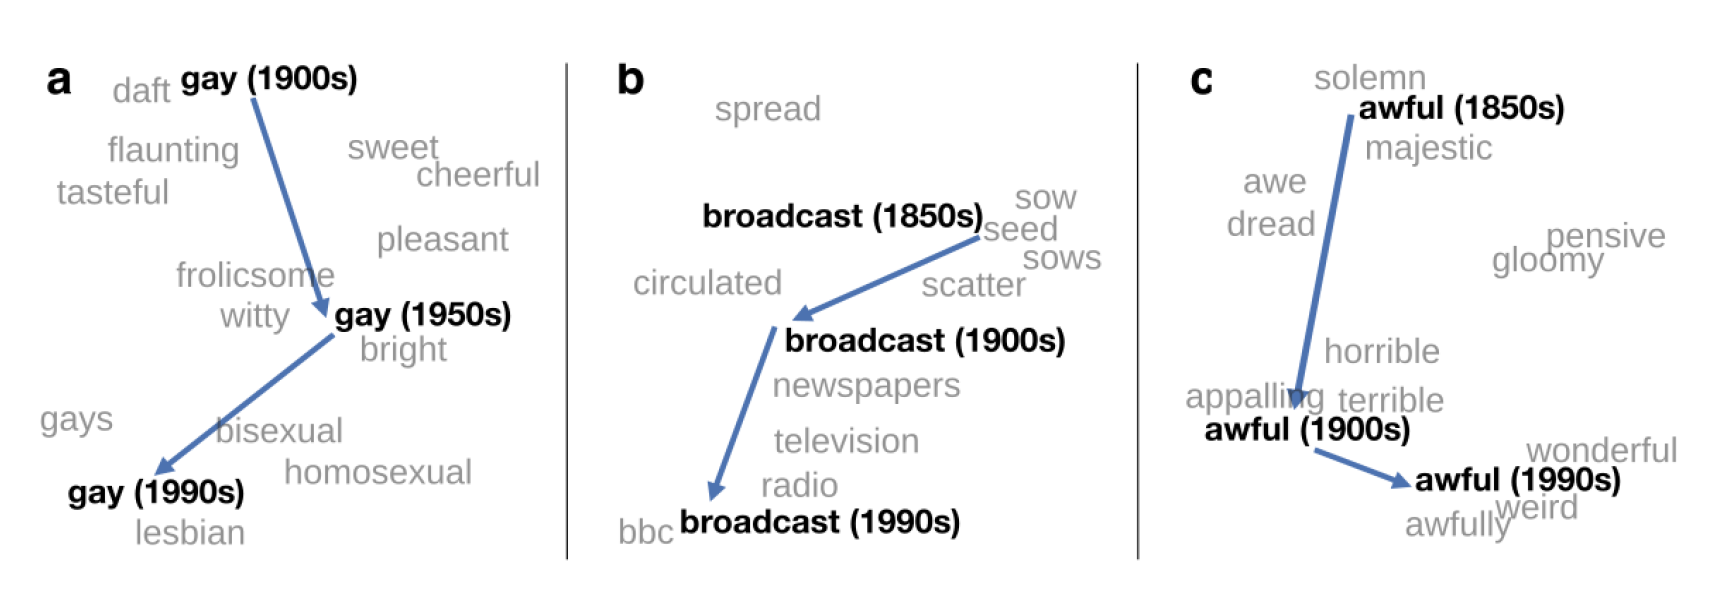
\includegraphics[width=0.95\textwidth,keepaspectratio]{figures_ref/Hamilton_et_al_2016_two_dimension_viz_of_semantic_change.png}
  \caption{Two-dimensional visualization of semantic change for the word \textit{gay}, \textit{broadcast}, and \textit{awful} (Adopted from \textcite{hamilton2016law})} \label{fig:hamilton}
\end{figure}

Semantic change is a manifestation of language use in both conventional and creative ways by the language community, making textual data temporal-dependent in essence \parencite{kutuzov2018survey}. As more attention is paid to the design of diachronic corpora and digitalization of historical text, a gap bridge and rapid advancements are seen in investigating semantic change in a data-driven way, especially from a distributional semantic perspective like diachronic word embeddings \parencite{kutuzov2018survey, tahmasebi2018survey, hamilton2016law, jawahar2019contextualized}.

Diachronic word embeddings make it possible to formulate or test hypotheses or laws of semantic change, establish temporal word analogy or relatedness, as well as discover semantic relations that are also changing over time. In \textcite{hamilton2016cultural}, linguistic drift and cultural shift can be also distinguished and measured based on diachronic word embeddings, with the latter restricted to a smaller set of neighboring words. With a growing interest in this research topic, insights have been made to highlight some key and challenging aspects of semantic change modeling \parencite{kutuzov2018survey,tahmasebi2018survey,camacho2018survey}.

For Classical Chinese, \textcite{li2020evolution} used the dependency parser trained on Kyoto Corpus of the Four Books to explore change of syntactic categories of Classical Chinese, yet a character-based analysis is adopted due to the segmentation issue of pre-modern Chinese. However, contrary to the assertion that pre-modern Chinese is mostly monosyllabic, the disyllabic development of Chinese has started as early as the Han dynasty \parencite{zhou2009,chang2008}, but the proposal by \textcite{lee2012classical} of the nested multi-level segmentation is able to reflect the complicated word segmentation challenge for languages like (pre-modern) Chinese \ascitedin{li2020evolution}. However, the results show that tokenizers such as MeCab-Kanbun and Stanza segment words by characters, and verbs like \zh{吃}{chī}{eat} or \zh{食}{shí}{eat} might be tagged as noun.

\subsection{Word-level Embeddings}
In Natural Language Processing, word embeddings are commonly added to the last layer of a deep learning model to translate discrete linguistic data to continuous numeric vectors. On the other, another line of research, referred to as ``corpus-centered'' approach in \textcite{antoniak2018evaluating}, focuses on the use of word embeddings as evidence for certain linguistic features or cultural characteristics. The topic of semantic change has directed attention to the use of corpora as inputs for diachronic word embeddings, or word-level embeddings in this study. Unsupervised lexical semantic change detection refers to the task dedicated to tracing semantic change based on diachronic word embeddings trained on time-sliced textual data or (sub)corpora. The modeling rests on the assumption that change in meaning is captured if change in word co-occurrences is identified.

One of the crucial steps of diachronic semantic modeling is the collection of texts and their temporal information in order to build word embeddings of different time epochs. Yet, diachronic corpora are subject to the lack of certain documents that are difficult to survive time and thus missing, which leads to the slow expansion of diachronic or historical corpora. The division of time periods, or the granularity, is also decided in the meantime of corpora compilation. Typically, the more recent the text is created, the more refined or specific the time units are set \parencite{kutuzov2018survey}. Among the diachronic textual data currently available, the main source includes but not limited to the Google Books Ngram Corpus\footnote{\url{http://books.google.com/ngrams}. A comprehensive review of diachronic corpora is provided by \textcite[38--41]{tahmasebi2018survey}.}, Corpus of Historical American English (COHA)\footnote{\url{https://www.english-corpora.org/coha/}}, Project Gutenberg Corpus\footnote{\url{https://www.sketchengine.eu/project-gutenberg-corpus/}} and self-compiled corpora with texts from newspapers and online social media.

While large-scale projects have led to the release of various pre-trained word embeddings, new ones continue to be trained to allow for more diversity and richness of the textual contents, and to adapt to specific research questions to be answered. This trend pertains to the definition of ``diachronic'', which highlights the characteristics of the source data with long stretch of time, and even from a long time ago in history.

Regarding conversational diachronic corpora, \textcite{giulianelli2019lexical} uses the r/LiverpoolFC corpus, which contains millions of words from posts about the English football team Liverpool from 2011 to 2017 on Reddit. Each utterance is annotated with a timestamp, and the dataset includes binary annotations of change on a list of selected words by the r/LiverpoolFC users themselves. The compilation of this corpus is based on sufficiently high temporal granularity, enabling the detection of abrupt shifts in the language use of a specific community. However, it is non-uniformly distributed, and thus it is more difficult to study changes in some of the time periods when a few user posts are generated.

In \textcite{hamilton2016cultural}, it is concluded that linguistically-driven semantic change occurs more slowly than a socially-motivated phenomenon. The invention of new technologies serves as prominent examples of cultural drift, as in \textit{apple} and \textit{cell}. Lists of words with the highest similarity scores or analogous pairs of words are analyzed to verify the results of diachronic word embeddings. The results on a full-scale vocabulary shows that a local measure of this partial list is sufficient to account for the phenomenon of a cultural drift.

\textcite{kutuzov2017tracing} exemplifies how social events such as armed conflicts are traced by monitoring word associations with ``anchor words'' like \textit{war}, \textit{peace}, and \textit{stable}. Another example is how \textit{president} becomes closer to \textit{Obama} during his term, as well as \textit{Israel's Prime Minister} and \textit{Christopher Nolan, The Dark Knight, 2008} \parencite{rosin2017learning} by finding continuous peaks of lowest distance between vectors with the dataset YAGO that contains temporal relations of named entities.

Nonetheless, the scarcity of ground-truth test data has made it difficult to evaluate the employed approach. The rating-based and dictionary-based collection of evaluation data are met with low inter-rater agreement of recruited annotators and/or inaccessibility of sources from the time period of interest \parencite{tang2018state}. \textcite{kutuzov2020uio} reveal that the results based on the test data can be distinctively varied across different languages. In contrast, evaluation datasets for Present-Day English are available, as well as translations and crowd-sourced human-annotated datasets in Mandarin Chinese.

In comparison with other approaches of semantic change detection, diachronic word embeddings exhibit a stronger explanatory power than frequency-based methodologies such as raw and relative frequency counts, as well as collocational analysis \parencite{kutuzov2018survey}. Indeed, it is convenient to manipulate word vectors, but past literature also presents the results and analysis in combination of the above two or more approaches to generalize the underlying principles of semantic change or echo with the proposed linguistic hypotheses \parencite{tahmasebi2018survey}.

In downstream applications, the importance of constructing temporal-aware embeddings as input data is acknowledged in the form of domain adaptation \parencite{huang2019neural}. Temporal adaptation is introduced as a form of domain adaptation to diachronic word embeddings and proves effective in the task of document classification \parencite{huang2019neural}. The presence and absence of documents, along with a smaller or less balanced corpus, has called for techniques like bootstrapping to mitigate the issue of variability \parencite{antoniak2018evaluating}.

Another challenge, namely the ``meaning conflation deficiency'', is brought up by \textcite{camacho2018survey}. Previously, word embedding technique is first implemented by \citeauthor{mikolov2013efficient} in \citeyear{mikolov2013efficient}. The embeddings models such as \gls{cbow}, \gls{sgns}, \gls{svdppmi} are static, for only one vector is generated to represent each word type in the diachronic textual data. Word-level vector representations do not account for the context of the keyword. Therefore, two words are likely to move closer toward each other in vector space not necessarily because they become semantically closer, possibly because one of the words undergoes meaning change on the sense level.

\subsection{Sense-level Embeddings}
In view of the static, context-independent nature of word embeddings, \textcite{hu2019diachronic} point out that the results do not show which sense has changed, and which remains stable, if not at a ``coarse-grained'' level. While static word embeddings rely on the analysis of neighboring words with the keyword to determine the presence or absence of meaning change, contextualized word embeddings mapped tokens to a possibly infinite sets of data points, allowing various methods to depict the subset of data, and are referred to as sense-level embeddings in this study. Pre-trained language models like ELMo and BERT are dynamic and context-dependent. Multiple embeddings can be extracted to represent a word in various contexts, thus allowing different senses of a word to be distinguished.

The pre-trained language models can be used in companion with sense inventories or cluster analysis. It is possible to produce mappings between contextualized word representations and sense descriptions from external linguistic resources (e.g. the Oxford English Dictionary) \parencite{hu2019diachronic}. Using the BERT pre-trained language model, \textcite{hu2019diachronic} track the evolution of English words from the year of 1810 to 2009 in the Corpus of Historical American English (COHA), and visualizes the interactions of the words' senses. The source texts from COHA are concordance lines which contain target words with a frequency of at least 10 times for over 50 consecutive years. Additionally, the sense identification task is performed by using example sentences in the Oxford English Dictionary (OED) as the knowledge base for similarity comparison with texts from COHA, and the total number of senses from the OED is 15836. Firstly, the last hidden layer of a target word's embedding is extracted from the pre-trained BERT language model. This token embedding is then compared with each sense representation retrieved from the OED word entry to determine which sense the target word belongs to.

Instead of sense inventories, various clustering algorithms are resorted to induce senses of target words, including $K$-Means and Gaussian mixture models \parencite{giulianelli2019lexical}. In \textcite{giulianelli2019lexical}, the target words are collected from \textcite{gulordava2011distributional} with annotated data on judgement task. Then, the cluster analysis reveals that different types of semantic change can be identified, including literal/metaphorical meanings, different senses of a polysemous word, words with different syntactic categories, and affixation. It is concluded that the change in sense distribution follows the ``S shape'' curve proposed in linguistics. Moreover, the actual uses of a certain sense can be inspected from the collected data. Their method is shown to be effective on the detection of short\text{-}term community\text{-}specific changes in word usages by including football data as the conversational corpus compared to diachronic corpus in their study. Their subsequent work is expanded to more languages and judgement data in the SemEval 2020 task \parencite{kutuzov2020uio}.

Notwithstanding, although context-independent and contextualized diachronic embeddings are proposed and explored in an increasing body of research to detect the presence of semantic change, which models are more capable of capturing this linguistic phenomenon remains an on-going topic that calls for evaluation methods for diachronic embeddings. It is debatable whether simpler models results in better performance \parencite{schlechtweg2019wind}.

Firstly, datasets like DURel (Diachronic Usage Relatedness)\footnote{\url{https://www.ims.uni-stuttgart.de/en/research/resources/experiment-data/durel/}} are established based on human ratings \parencite{schlechtweg2018diachronic} and word injection \parencite{schlechtweg2019wind}, which is based on similar concepts like domain-specific word sense disambiguation or term ambiguity detection, inspired by term extraction and synchronic version of SURel (Synchronic Usage Relatedness)\footnote{\url{https://www.ims.uni-stuttgart.de/en/research/resources/experiment-data/surel/}} where variation lies in sense divergence across domains for research topics like online language analysis.

However, evaluation data are scarce \parencite{wevers2020digital}, and hand-picked attested examples from literature or dictionaries with tags like ``obsolete'' \parencite{hamilton2016cultural} have proven that automatic semantic change detection is able to capture semantic change \parencite{schlechtweg2019wind} (As previously shown in \tref{tab:use_case}), but the results still vary depending on the test or evaluation data that are currently available.

For example, the exploration of semantic change laws has proved influential in the latest researches, the synchronic or ``within-time-period'' accuracy still has to rely on the test data that are available for a certain period of time. In \textcite{hamilton2016law}, the anchoring time period is the 1990s for the diachronic corpora of Google Ngrams from the year of 1800 to 2009. Additionally, the result of \textcite{schlechtweg2019wind} shows that \gls{sgns} with orthogonal Procrustes alignment achieves the highest performance based on the DURel dataset, whereas topic modeling has the least correlation with the examined dataset. Furthermore, the results in \textcite{schlechtweg2019wind, dubossarsky2017outta} shows that cosine distance (global neighborhood distance) outperforms local neighborhood distance under the condition of aligned embeddings, and the results of topic modeling is sensitive to corpus size and frequency of the target words, which makes it a less desirable method in diachronic semantic modeling.

\section{Visualizing Semantic Change}
After the training of diachronic embeddings, if the embeddings are separately trained, they are are randomly initialized, and it is necessary to align them in the same vector space \parencite{hamilton2016law}. To put it differently, the alignment of embeddings leads to the comparability of the vectors representing the same target word from different time periods. To project separately trained word embeddings, linear transformation, distance-preserving projection, second-order embeddings that consist of vectors of the similarity scores of the target word to its neighboring words, are used. The most widely adopted alignment algorithm is proposed by \textcite{hamilton2016law}, who utilizes the orthogonal Procrustes analysis to display datapoints from different embeddings models in the same vector space.

In addition to the alignment of separately trained embeddings, temporal referencing (TR) \parencite{dubossarsky2019timeforchange} is proposed to mitigate the noise issue induced by alignment. Because of alignment, the results, especially low-frequency words, are influenced by noises \parencite{dubossarsky2019timeforchange,dubossarsky2019timeout}. However, the lack of widely-accepted evaluation procedures have made it difficult to learn more about the noises invited by vector space alignment \parencite{dubossarsky2019timeout}. Another line of research resorts to jointly learning word representations of all time periods by incrementally updating the model. Furthermore, the Hierarchical Softmax function is introduced to improve the efficiency of the updating.

In view of the scale of data, semantic change modeling is evaluated on two grounds--the combination of statistical tests and visualizations, as well as classification tasks \parencite{tang2018state}. To visually display the trained embedding models, high-dimensional visualization techniques are employed to assess the results of the word representation learning \parencite{liu2017visual}. Visualization of diachronic data allows researchers to explore any target word to see how the data changes along with time.

To visualize the results, vectors originally trained in high-dimensional space are transformed and projected in two or three dimensions. \gls{pca} and \gls{tsne} \parencite{vandermaaten2008tsne} are two common methods of dimensionality reduction. Using the former, only the most influential dimensions are retained, while the latter reflects more geometrical structure of the high-dimensional data because it is non-linear \parencite{vandermaaten2008tsne}.

However, the exploration of the internal structure and properties of an embedding is generally non-interactive \parencite{smilkov2016projector}. In \citeyear{smilkov2016projector}, Google releases the Embedding Projector under the TensorBoard framework (See \fref{fig:tensorboard_demo}), which provides users with many interactive functionalities such as zooming, filtering, inspection of data points with metadata created in the table format by users \parencite{smilkov2016projector}\footnote{Web-based demonstration of interactive graphical representation of high-dimensional embeddings via Google's TensorBoard Embedding Project can be visited at \url{https://projector.tensorflow.org}}.

\begin{figure}[H]
  \centering
  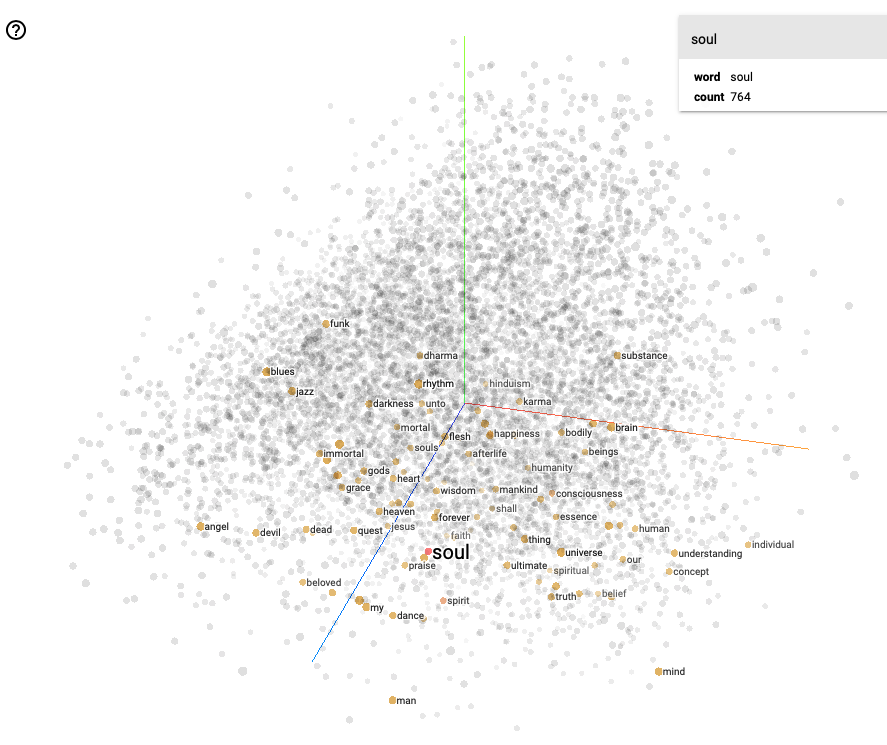
\includegraphics[width=0.85\textwidth,keepaspectratio]{figures_ref/embedding_projector_demo}
  \caption{Visualizing data using the Embedding Projector in TensorBoard} \label{fig:tensorboard_demo}
\end{figure}

Particularly, \textcite{coenen2019visualizing} recognizes the adaptability of BERT to various downstream tasks and the possibility of the language model to extract useful features from raw textual data. To understand the internal structure of BERT and how discrete linguistic units are translated into continuous numeric vectors, the UMAP visualization of the token vectors and nearest-neighbor classifier are used, as shown in \fref{fig:coenen_umap}. Semantically, fine-grained sense information is encoded in BERT, even in low-dimensional subspace. \textcite{coenen2019visualizing} concludes that both semantic and syntactic information are encoded in the contextualized embeddings in ``complementary subspaces.'' Yet, an attention-based model like BERT does not necessarily ``respect semantic boundaries when attending to neighboring tokens, but rather indiscriminately absorb meaning from all neighbors'' \parencite{coenen2019visualizing}.

\begin{figure}[H]
  \centering
  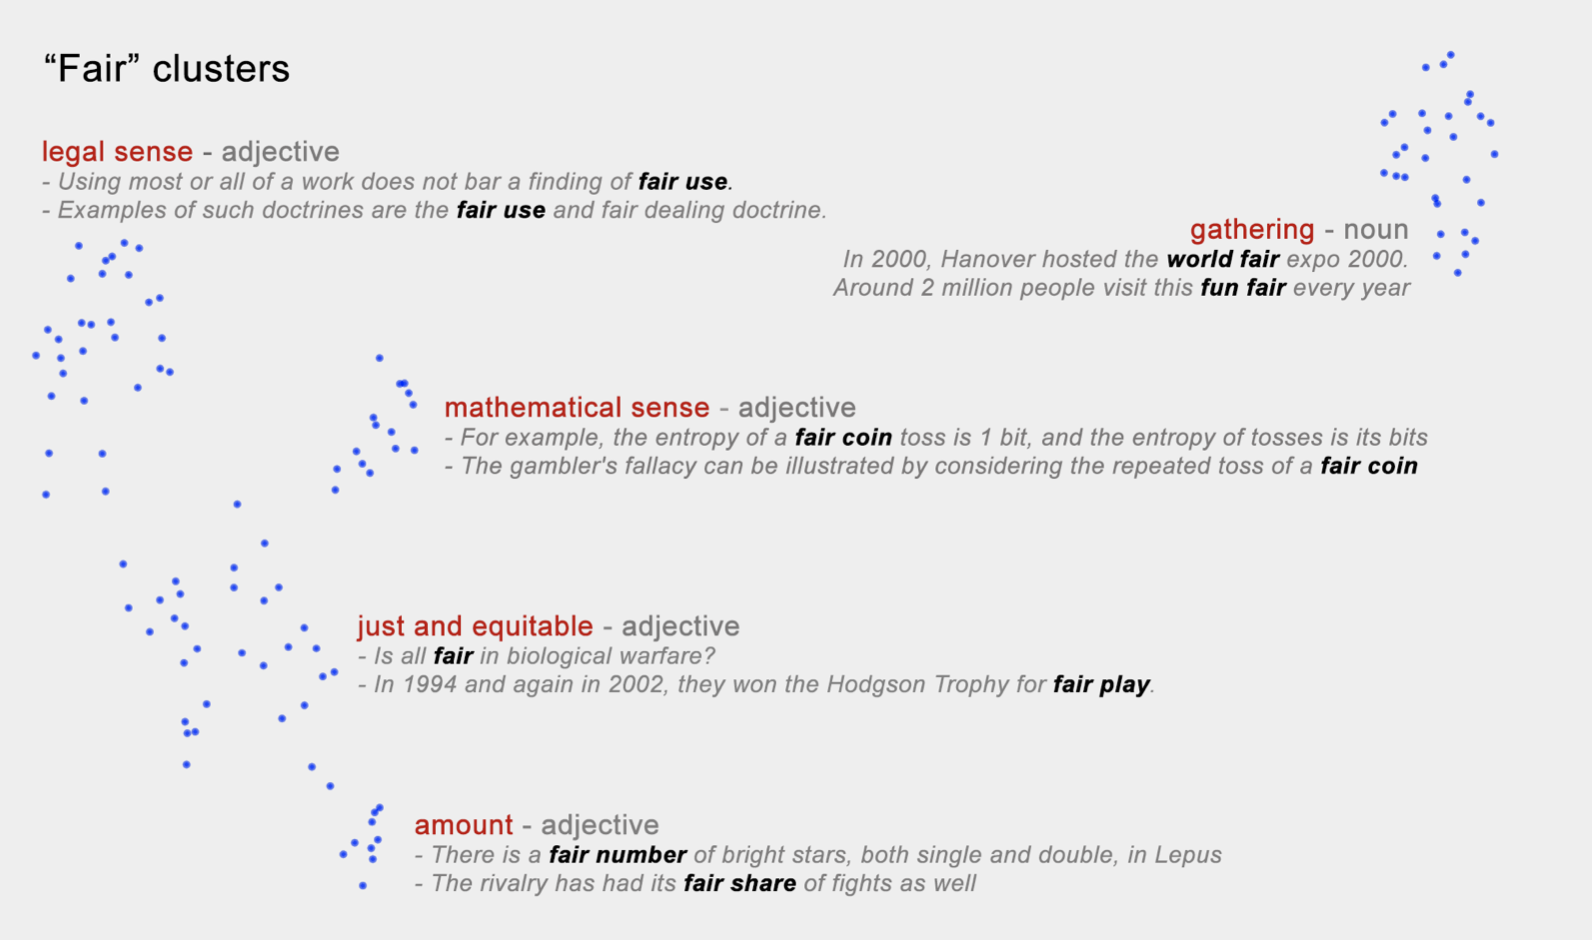
\includegraphics[width=0.85\textwidth,keepaspectratio]{figures_ref/coenen_umap}
  \caption{Visualizing contextualized embeddings using UMAP with the word \textit{fair} as an example (Adopted from \textcite{coenen2019visualizing})} \label{fig:coenen_umap}
\end{figure}

% \begin{figure}[H]
%   \centering
%   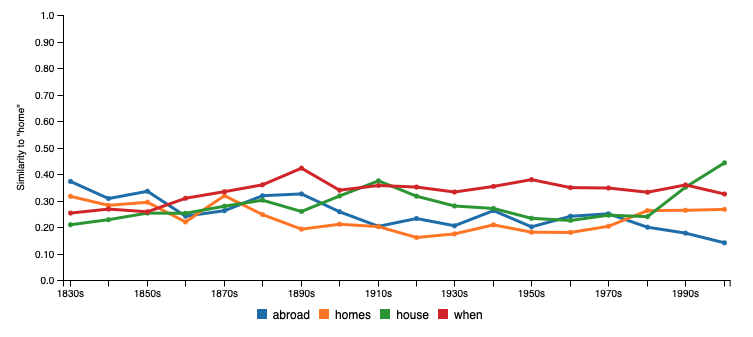
\includegraphics[width=0.85\textwidth,keepaspectratio]{figures_ref/jeseme_similar_words}
%   \caption{Visualizing similar words of \textit{home} in the Corpus of Historical American English (COHA) in JeSemE (Adopted from \textcite{hellrich2017exploring})} \label{fig:jeseme_similar_words}
% \end{figure}

\section{Laws of Semantic Change}
The application of computational linguistics to historical semantics bears fruit of inspiring works on generalizations of semantic change. It is hoped that computational analyses would help explain the mechanisms of semantic change such that a level of maturity like laws of sound change could be reached. Instead of examining instances of semantic change, it becomes more and more computationally feasible and efficient to analyze this linguistic phenomenon on a large scale. The degrees of semantic change are quantitatively measured and how other linguistic factors play a role in semantic change is revealed, which motivates the research inquiries of testing the results against laws of semantic change that have been proposed in theory or observed on a smaller scale. Among them are the law of prototypicality \parencite{dubossarsky2015bottom}, the law of conformity \parencite{hamilton2016law}, and the law of innovation \parencite{hamilton2016law}. The competing laws of parallel change and differentiation are reviewed in \textcite{xu2015computational}.

Based on the English lexicon between 1850 and 2009 in the Google Ngram corpus, \textcite{dubossarsky2015bottom} find that lexical semantic change positively correlates with the centroid of a word's cluster, which is symbolic of the word's prototype, hence the ``law of prototypicality.'' $K$-means clustering, with varying numbers of clusters, is applied to a list of most frequently used words in the Google Ngram corpus. Within the same cluster, words that undergo a higher degree of semantic change are located farther from the cluster's centroid.

A further analysis reveals that a cluster's centroid has a stronger correlation than a prototypical exemplar, which is the second closet to the centroid. Observing this tendency, the authors argue that this finding enables an exploration of semantic change in relation to a hypothetical, abstract, non-lexicalized prototypical member. In addition, it is found that the correlation increases as the number of clusters increases, but drops once the number of clusters reaches a maximum, suggesting that the boundaries of semantic categories can be drawn. Therefore, this research offers a bottom-up analysis of the diachronic prototypical semantics with flexible boundaries of semantic categories to evaluate a large number of lexical items.

The laws of conformity and innovation are put forward by \textcite{hamilton2016law}. The former posits that observed frequency negatively correlates with the rate of semantic change, while the latter asserts that semantic change is positively influenced by a word's polysemy, the number of a word's senses, in controlled frequency. Polysemy is measured through contextual diversity from the co-occurrence network of the trained diachronic embeddings, which is also the reason why the relationship between polysemy and the rate of semantic change is examined under controlled frequency due to the intrinsic correlation between the two variables.

To evaluate the two laws, known instances of semantic change from literature and top 10 words from the experiment results are reviewed. The Spearman correlation is then calculated on a full scale between the rate of semantic change and the two linguistic factors, namely a word's observed frequency and number of senses, for 4 languages (English, German, French, Chinese), and 6 historical corpora (Google books in all genres for the 4 selected languages, an additional corpus from Google books in the fiction category, and COHA), which span 2 centuries (1800--2009) at the interval of a decade. 

Nonetheless, the judgement of synchronic accuracy has to rely on the time period of 1990s possibly because the test data for earlier time periods are rare, as pointed out to be an issue of diachronic semantics studies \parencite{wevers2020digital}. Yet, the quantification of the rate of semantic change through computational analysis is inspiring. It is revealed that the two laws of semantic change are proportional in the form of a power law. Additionally, the consideration of controlled frequency is crucial because the results show complementary trends for the two laws of semantic change examined if untreated.

In \textcite{xu2015computational}, near-synonyms are shown to change in parallel, and thus the law of parallel change is more favorable than the law of differentiation. That is, these two laws attempt to characterize whether words with similar meanings continue to be similar, or turn out to be divergent. Nouns, verbs, and adjectives are extracted from the Google Ngram corpus from 1890 to 1999. The selection of synonyms and control pairs is determined by external sources like thesauri and WordNet sense inventories and the computation of the Jensen-Shannon (JS) divergence scores, with a lower score representing a higher similarity in meaning.

To further prevent bias from different lists of control pairs, the analysis by \textcite{xu2015computational} is conducted chronologically as well as in reserved time order. The degree of semantic change is then derived from the intersection of nearest neighbors between two time periods, and the results are consistently in favor of the law of parallel change against that of differentiation. Yet, although this research is often referenced in subsequent works on computational analyses of semantic change, the meaning vectors are not constructed from word embeddings, but frequency tables of the target word with words within 1 window size.

With the accumulation of related researches, not only are laws of semantic change examined by inspecting the relations between the degree of semantic change and various linguistic factors, the use of word embeddings itself as a method for diachronic linguistic studies are also evaluated. The results have shown to be helpful in the development of semantic change generalizations and principles. However, different conclusions might exist given different experiment settings and source data, so no consensus has been reached regarding a wider generalization of semantic change in more languages building upon diachronic word embeddings.

\end{document}

% conferences:
% SemEval
% NLP for semantic change (https://semanticshifts.sciencesconf.org/data/pages/Course12.pdf)
% https://driftselection-evolang2020.github.io/#submission_(ended)